\documentclass[12pt, a4paper]{article}
\usepackage[utf8]{inputenc}
\usepackage{hyperref}
\usepackage[left=1.00in, right=1.00in, top=1.00in, bottom=1.00in]{geometry}
\usepackage{graphicx}
\usepackage{xcolor}
\graphicspath{ {./} }
\title{CS348 Project - Final Report}
\author{Abdullah Bin Assad\and Chandana Sathish \and Lukman Mohamed \and Vikram Subramanian \and Dhvani Patel \\}
\begin{document}
\maketitle

\begin{center}

    \url{https://watch-dog.azurewebsites.net/}
\end{center}
\section*{Application description}
\subsection*{Application User}
We have created an interactive web app for people interested in exploring crime data in the Greater Toronto Area. People who wish to assess how safe a neighbourhood is before investing in a new property or novice drivers trying to avoid accident-prone roads or just people curious about crime rates around them can greatly benefit from our application.
\subsection*{Interaction with the app}
A user would simply search for a query (as seen on the demo application) using the drop-down on certain words in the question to tailor the search to their needs. For example, “I want to explore bicycle theft crimes in 2019 (year) citywide on a bar chart” can be one of the many queries a user selects. Alternatively, a user can also pick from a list of predefined queries if they are unsure about where to start. Once the user clicks “OK”, the page updates to display the requested query and allows them to change the representation/visualization of the data as well as further refine their search with more options. We also plan on adding additional features as follows.
\subsection*{Key features}
\begin{enumerate}
\item Filter crime/traffic events (starter question with drop-down for filtering different columns as seen in demo) and show results on a table
\begin{itemize}
    
    \item Filter by crime indicator
    \item Filter by year/month
    \item Filter by neighbourhood
\end{itemize}
\item Display crime data
\begin{itemize}
\item bar chart, line chart, and pie chart
\item map, heat map

\item summary/total count
\end{itemize}
\item Create predefined complex queries in the form of question and answer
\begin{itemize}
    \item Example - At what hour do most crimes occur, which neighbourhood has the most number of traffic accidents, is there a correlation between education/demographic and crime, etc.
\end{itemize}
\item Provide users with information on which police division they are situated closest to based on the address they provide us with
\item Report a crime
\item Interactive “How well do you know your city” feature
\begin{itemize}
    \item Let the user guess certain values from a query they select, then show them the actual results and tell them how close they were
\end{itemize}
\end{enumerate}
\subsection*{Data}
The tables we get from the Toronto Police Open Data:
\begin{itemize}
    \item \url{https://data.torontopolice.on.ca/pages/open-data}
\end{itemize}

We get a few additional columns of the census from the Toronto City Open Data:
\begin{itemize}

 \item \url{https://open.toronto.ca/dataset/neighbourhood-profiles/}
\end{itemize}
\color{black}
The tables themselves are a little difficult to work with. Therefore, we create a data parser (in code.zip) to convert it to .csv files that fulfill our requirements. Sample data and production data are part of the code.zip as csv files (ex. Neighbourhood.csv, CrimeEvent.csv).
\subsection*{System support}

\hspace{\parindent}Our interface consists of an interactive web-app. Both the web application and the SQL database are hosted on Microsoft Azure. Azure AppServices and MySQL are modern, scalable, efficient and flexible. This setup is ideal and efficient for building a web app such as ours; plus Azure is cheaper than the alternatives. 

The back end is made up Node.js + Express.js from which API end points are exposed. This is what directly talks with the database. The front end is a React application.  \color{blue}The notalable NPM packages used include: the Semantic UI React library for UI components, the Mapbox API for the maps you see in the application, ChartJS and D3.js for the data presentation, and ag-grid for the table.\color{black} Thus, our web application code mostly consists of JavaScript. Members of our group have experience with Node.js and React which gave us an excellent basis for our project.


\section*{Design database schema}
\subsection*{List of assumptions}
\begin{itemize}
    \item all reported times of incidents are either in or after 2014
    \item for regular crimes and traffic accidents, the time and place of the incident are recorded accurately and not left out (not NULL mostly)
    \item the level and standard of reporting crimes is consistent in all neighbourhoods (required for useful analysis and comparison among neighbourhoods)
    \item the cause of the traffic accident is taken from testimonies of all parties involved and is not one sided (although hard to avoid survivorship bias)
    \item the police arrive at the scene of an accident within reasonable time to be able to assess the road conditions leading up to the cause of the accident
    \item all parties involved in an accident are accounted for (driver, passengers, pedestrians)
    \item the status of stolen bikes is updated as best as possible (most bikes are never recovered)
\end{itemize}

\subsection*{E/R diagram}
\color{black}
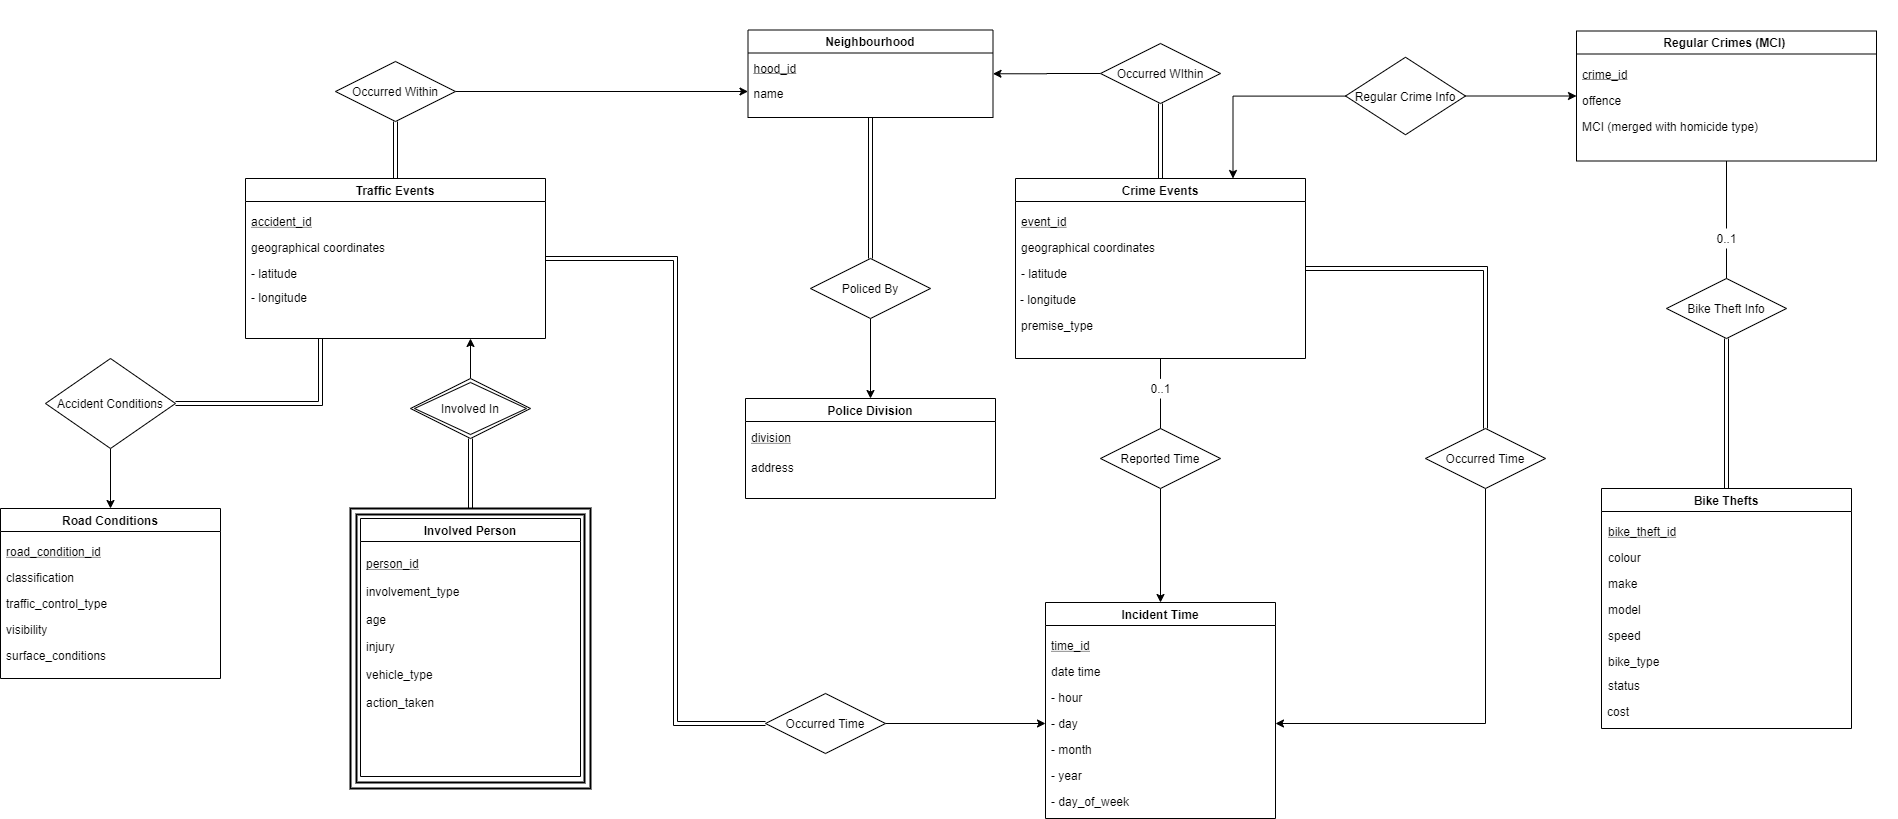
\includegraphics[scale=0.3]{ER Diagram.png}
Note: Check the standalone image of the ER diagram if this one is too small.
\subsection*{Relational Data Model}
\begin{itemize}
    \item IncidentTime
    \begin{itemize}
        \item \underline{time\_id} : INT 
        \item hour : INT
        \item day : INT 
        \item month : INT
        \item year : INT
        \item day\_of\_week : INT
    \end{itemize}
    \item PoliceDivision
        \begin{itemize}
        \item \underline{division} : INT
        \item address : VARCHAR(50)
        \item area : DECIMAL(12, 9)
        \item shapeLeng : DECIMAL(12, 6)
        \item shapeArea : DECIMAL(11, 3) 
    \end{itemize}
    \item Neighbourhood
        \begin{itemize}
        \item \underline{hood\_id} : INT
        \item name : VARCHAR(50) 
        \item employment\_rate : DECIMAL(4, 2) 
        \item high\_school : DECIMAL(4, 2) 
        \item university : DECIMAL(4, 2)
        \item technical\_degree : DECIMAL(4, 2)
        \item division : INT (Foreign Key Referencing  PoliceDivision(division))
    \end{itemize}
    \item BikeTheft
        \begin{itemize}
        \item \underline{event\_id} : INT (Foreign Key Referencing CrimeEvent(event\_id))
        \item colour : VARCHAR(50)
        \item make : VARCHAR(50)
        \item model : VARCHAR(50)
        \item speed : VARCHAR(50)
        \item bike\_type : VARCHAR(50)
        \item status : VARCHAR(50)
        \item cost : DECIMAL(8, 2)
    \end{itemize}
    \item RegularCrime
        \begin{itemize}
        \item \underline{crime\_id} : INT
        \item offence : VARCHAR(50)
        \item MCI : VARCHAR(50)
    \end{itemize}
    \item CrimeEvent
        \begin{itemize}
        \item \underline{event\_id} : INT
        \item occurrence\_time\_id : INT (Foreign Key Referencing IncidentTime(time\_id))
        \item reported\_time\_id : INT (Foreign Key Referencing IncidentTime(time\_id))
        \item crime\_id : INT (Foreign Key Referencing RegularCrime(crime\_id))
        \item hood\_id : INT (Foreign Key Referencing Neighbourhood(hood\_id))
        \item latitude : DECIMAL(10,8)
        \item longitude : DECIMAL(11,8)
        \item premise\_type : VARCHAR(50)
    \end{itemize}
    \item InvolvedPerson
    \begin{itemize}
        \item \underline{accident\_id} : INT (Foreign Key Referencing TrafficEvent(accident\_id))
        \item \underline{person\_id} : INT
        \item involvement\_type : VARCHAR(50)
        \item age : INT
        \item injury : VARCHAR(50)
        \item vehicle\_type : VARCHAR(50)
        \item action\_taken : VARCHAR(50)
    \end{itemize}
    \item RoadCondition
    \begin{itemize}
        \item \underline{road\_condition\_id} : INT
        \item classification : VARCHAR(50)
        \item traffic\_control\_type : VARCHAR(50)
        \item visibility : VARCHAR(50)
        \item surface\_condition : VARCHAR(50)
    \end{itemize}
    \item TrafficEvent
    \begin{itemize}
        \item \underline{accident\_id} : INT
        \item occurrence\_time\_id : INT (Foreign Key Referencing IncidentTime(time\_id))
        \item road\_condition\_id : INT (Foreign Key Referencing RoadCondition(road\_condition\_id))
        \item hood\_id : INT (Foreign Key Referencing Neighbourhood(hood\_id))
        \item latitude : DECIMAL(10,8)
        \item longitude : DECIMAL(11,8)
    \end{itemize}
\end{itemize}
\color{blue}
\subsection*{Application Overview}
\color{black}
\begin{itemize}
    \item Starter Question
    \begin{itemize}
        \item Located at very top of the application .
        \item It filters the information in the cards below by crime type (regular crimes, bike thefts and traffic accidents). 
        \item  For crimes we have filters for the major crime indicator (MCI), date (year or month) and location (citywide, neighbourhood and police division). 
        \item By default, it is set to show all crimes citywide (Toronto) that happened in 2019.
        \item Click OK and the userr new search will update the cards below.
    \end{itemize}
    \item Data Cards
    \begin{itemize}
        \item All queries have similar cards with different data.
        \item Table Card
        \begin{itemize}
            \item Located right below the Starter Question.
            \item Contains the raw data from the query.
            \item Paginated and filterable.
        \end{itemize}
        \item Heat-map Card
        \begin{itemize}
            \item Located right below the Table Card.
            \item Shows the amount of crimes per time period. 
            \item Interact to refine the time range.
        \end{itemize}
        \item Summary Card
        \begin{itemize}
            \item Shows the number of crimes per major crime indicator. 
        \end{itemize}
        \item Cluster Map Card
        \begin{itemize}
            \item Shows each individual crime location. 
            \item We can zoom in on the cluster to break it up and see individual locations.
        \end{itemize}
        \item Line Chart Card
        \begin{itemize}
            \item Shows the number of crimes per month if our date type is set to year, or day if our date type is set to month.
        \end{itemize}
        \item There are a few other data cards besides the ones mentioned above: horizontal bar char, a doughnut chart, and a pie chart.
        \item Note that, since it may be hard to view certain small numbers, the user can click on a chart label to remove it.
        \item Bike Thefts and Traffic Incidents
        \begin{itemize}
            \item Have the same cards.
            \item As different types of data are collected for different types of crimes, different types of data are mentioned in the above data cards.
        \end{itemize}
    \end{itemize}
    \item Police Division Map
    \begin{itemize}
        \item Located below everything mentioned above. 
        \item Shows the amount of crimes per police division and where the police divisions are located.
        \item Provide an address and the application will output the closest police division.
    \end{itemize}
    \item Additional Filters
    \begin{itemize}
        \item A few filters are used in the application. 
        \item For example, we can look at the robberies that happened in rexdale-kiplin in March 2018.
        \item We can also filter by a police division instead.
    \end{itemize}
    \item Report Crime
    \begin{itemize}
        \item Located at the bottom right of the application.
        \item Fill this out to report a crime and update the database.
        \item Please recall that the userr new crime will be added to 2020 (so update the filter before checking!).
    \end{itemize}
    \item Batman Mode
    \begin{itemize}
        \item The button to activate it is located at the top right of the application.
        \item A game that tests how well the user know the city of Toronto and its crime. 
        \item Once activated, the user has to guess the total number of crimes that occurred and the crimes per month/day for the selected query.
        \item Then at the end, users can see their score for guessing both the data.
        \item This is a fun way for users to explore the data and challenge their friends.
    \end{itemize}
    \item Predefined Queries
    \begin{itemize}
        \item Located at the same spot as the Starter Question.
        \item An alternative to the Starter Question if the user is not sure what they are looking for.
        \item Select the toggle to the left of the Starter Sentence to switch to Predefined Queries.
        \item Currently we have 21 queries, but more can be added quite easily.
    \end{itemize}
\end{itemize}
\color{blue}
\subsection*{Changes/Improvements Since Milestone 2}
\color{black}
\begin{itemize}
	\item Created additional indices to speed up queries for the predefined questions feature (2.4 seconds to 0.6 seconds!):
	\begin{itemize}
		\item CREATE INDEX MCI ON RegularCrime(MCI);
		\item CREATE INDEX BikeType ON BikeTheft(bike\_type);
		\item CREATE INDEX InvolvedPersonType ON InvolvedPerson(involvement\_type);
	\end{itemize}
	\item Implemented all remaining features and polished application
\end{itemize}
\end{document}